\documentclass{article}
\title{The microscopic structure of materials}
\author{Izaak van Dongen}
\usepackage{amsmath}
\usepackage{amsfonts}
\usepackage{graphicx}
\usepackage{savetrees}

\graphicspath{ {images/} }

\usepackage{amsthm}
\usepackage[framemethod=tikz]{mdframed}

\begin{document}
    \section{Metals (2)}
    \subsection{Definitions}
%    \begin{mdframed}[backgroundcolor = gray!30,
%        frametitle = Crystalline]
%        Particles are arranged in a regular lattice
%    \end{mdframed}
%    \begin{mdframed}[backgroundcolor = gray!30,
%        frametitle = Polycrystalline]
%        There are different crystalline grains
%    \end{mdframed}
%    \begin{mdframed}[backgroundcolor = gray!30,
%        frametitle = Grain]
%        A single crystalline subsection of a polycrystalline material
%    \end{mdframed}
%    \begin{mdframed}[backgroundcolor = gray!30,
%        frametitle = Grain boundary]
%        The boundary between grains
%    \end{mdframed}
%    \begin{mdframed}[backgroundcolor = gray!30,
%        frametitle = Lattice]
%        A regular (square) array of particles
%    \end{mdframed}
    \begin{mdframed}[backgroundcolor = gray!30,
        frametitle = Slip plane]
        A two-dimensional plane in which slip occurs - this is aligned with a
        dislocation
    \end{mdframed}
    \begin{mdframed}[backgroundcolor = gray!30,
        frametitle = Lattice defects]
        Imperfections/irregularities in the regular lattice structure. Examples
        include the dislocation.
    \end{mdframed}
    \begin{mdframed}[backgroundcolor = gray!30,
        frametitle = Dislocations]
        A missing particle in a lattice structure, which allows slip to occur
    \end{mdframed}
    \begin{mdframed}[backgroundcolor = gray!30,
        frametitle = Alloys]
        Compounds of multiple metals. Alloys are often strong as alloy
        particles can ``pin'' dislocations.
    \end{mdframed}
    \subsection{Crystallinity}
    A crystalline structure means that ``individual particles are arranged in a
    regular pattern over distances many times the spacing between the
    particles'' \cite[p.~96]{OCRPhysics}. The important thing is the existance
    of some regular structure. Such a regular square grid may also be called a
    lattice - these can be used pretty much interchangeably. Most metals, in
    addition to \textit{crystals} and ionic compounds, are crystalline in
    structure.
    \begin{figure}[h]
        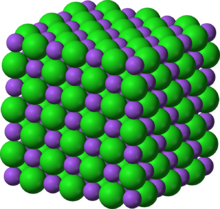
\includegraphics[width=0.1\textwidth]{crystal}
        \centering
        \caption{A 3-D NaCl crystal}
    \end{figure}
    \subsection{Polycrystallinity}
    A ``polycrystalline'' material ``consists of a number of grains all
    oriented differently relative to one another but with an ordered, regular
    structure within each individual grain.'' \cite[p.~98]{OCRPhysics}. Here a
    grain is a part of the material, on the microscopic level, which is like a
    single ``proper'' crystal. The boundary between grains is called the
    ``grain boundary``.
    \begin{figure}[h]
        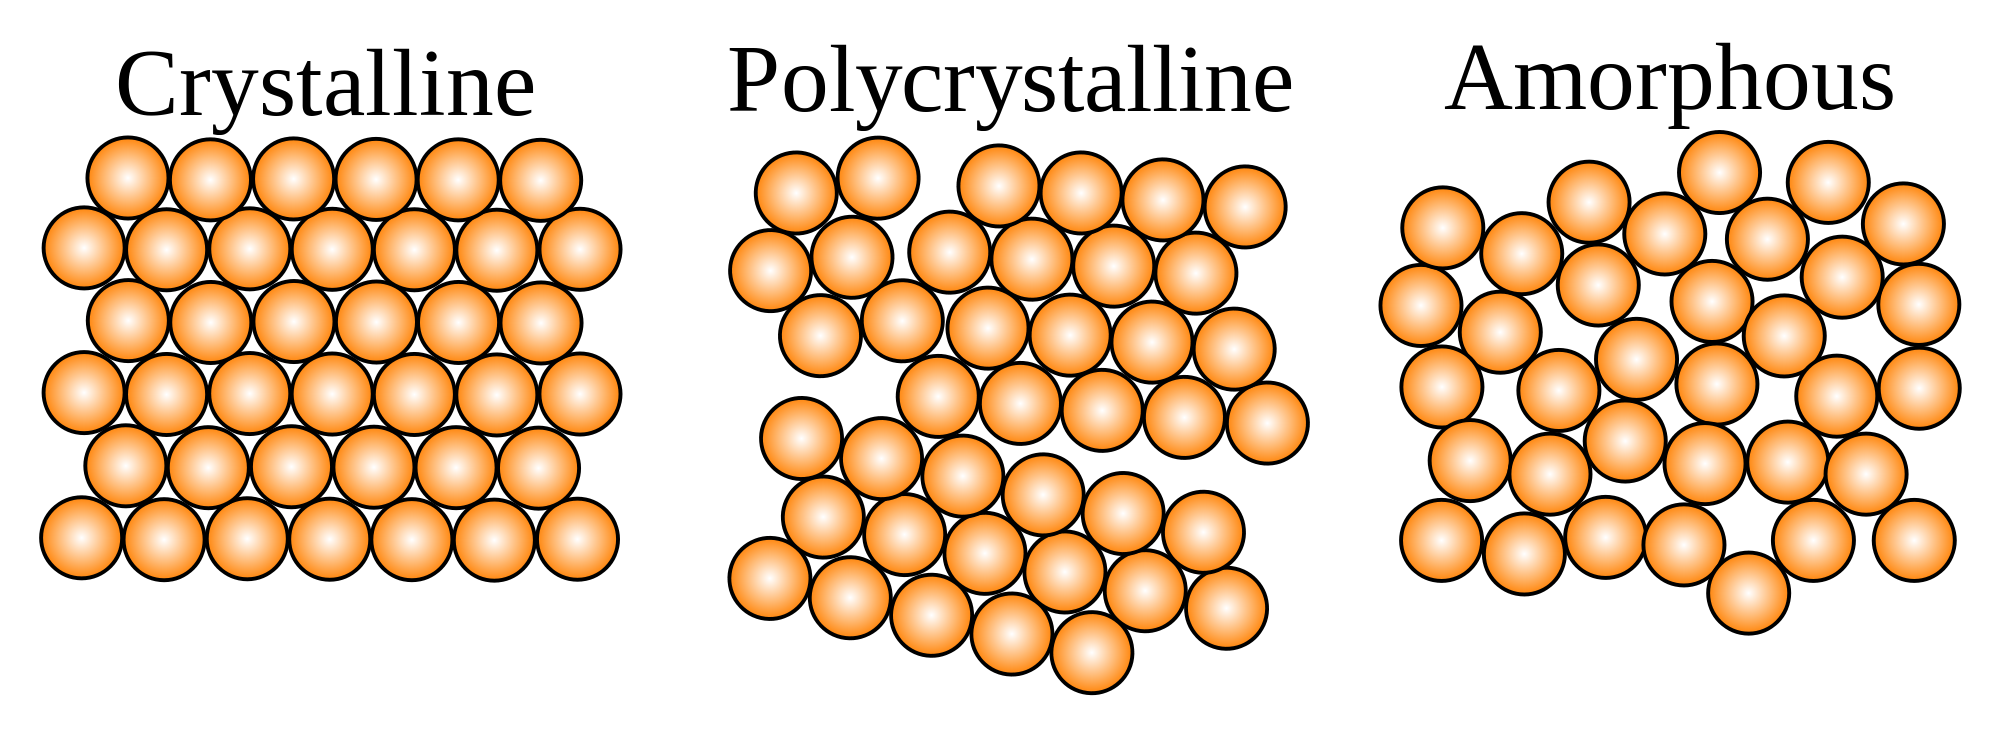
\includegraphics[width=0.5\textwidth]{crystal_and_poly}
        \centering
        \caption{Crystallinity vs. polycrystallinity}
    \end{figure}
    \subsection{Dislocation}
    A dislocation is a ``mismatch in [a] regular row of atoms''
    \cite[p.~96]{OCRPhysics}. Dislocations allow atoms to slide, or ``slip''
    over one another. This happens in a certain plane, which is called the
    ``slip plane``.
    \begin{figure}[h]
        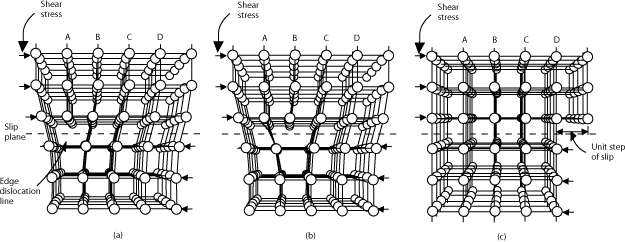
\includegraphics[width=0.5\textwidth]{dislocation}
        \centering
        \caption{Dislocation and slipping}
    \end{figure}
    This process of slipping accounts for why metals are relatively malleable
    and ductile, as only a couple of atoms have to be ``moved'' - if metals
    were ideal crystals, whole layers of atoms would have to be moved to deform
    the metal.
    
    The fact that they are malleable also results in metals being tough, ie are
    very unlikely to shatter when they break. This is because, as they are
    malleable, cracks will just become blunt and stretch when subjected to
    stress, rather than propagate, as they might in a ceramic.
    \subsection{Alloys}
    An alloy is a ``metal made by combining two or more metallic elements''.
    Alloys are often stronger than just metals, and this can be explained in
    terms of slipping. Alloy atoms can "pin" a dislocation, preventing slip.
    \begin{figure}[h]
        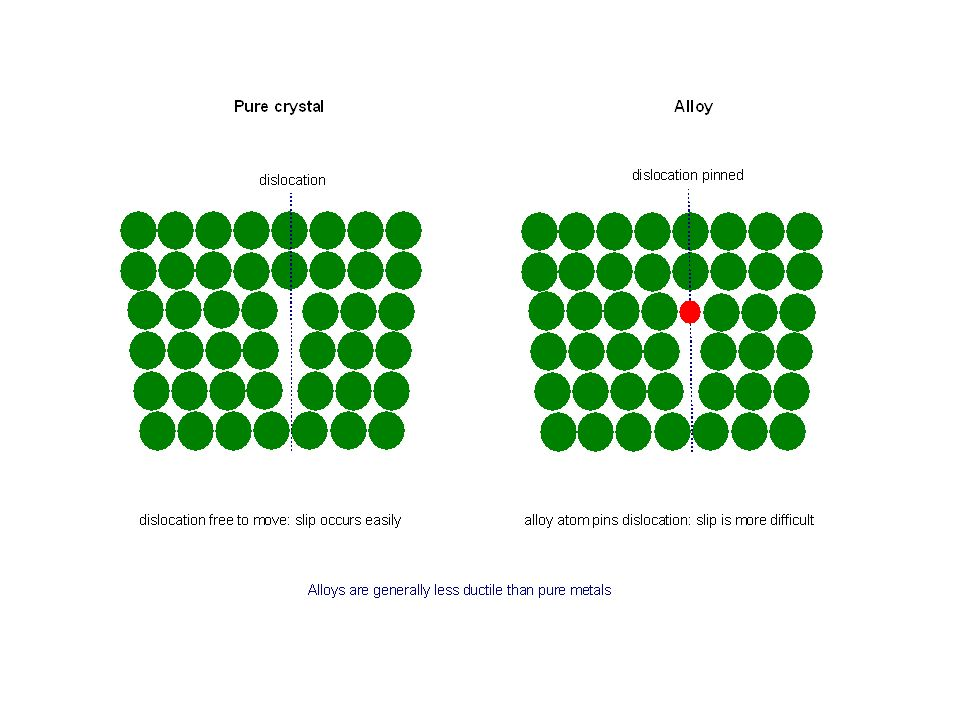
\includegraphics[width=0.5\textwidth]{alloy}
        \centering
        \caption{Pinned dislocation in an alloy}
    \end{figure}
    \subsection{Pure crystals}
    Sometimes a pure crystal is desired. Solids are often made by cooling
    liquids until they freeze. Liquids are amorphous, so by quickly cooling
    them, the amorphousness of the liquid is ``captured'' and the resulting
    solid isn't very crystalline. Cooling them more and more slowly can yield
    more crystalline structures, with fewer dislocations. A very pure crystal
    can be made simply by cooling a liquid very slowly.

    An example of this is high-purity silicon used in microchips. Here silicon
    is used as a semiconductor \cite{SOSilicon}, so it should be as pure as
    possible to maximise its conductivity and hence the performance of the
    chip.
    \subsection{Other lattice defects}
    Other lattice defects can also occur. One of these is a ``vacancy''. This
    is when ``an atom is missing from its lattice point ''
    \cite{LatticeDefects}.  The result of a vacancy is that ``there is a change
    in the coordination of atoms around the defect. This means that the forces
    are not balanced in the same way as for other atoms in the solid, which
    results in lattice distortion around the defect'' \cite{VirginiaDefects}.
    \begin{figure}[h]
        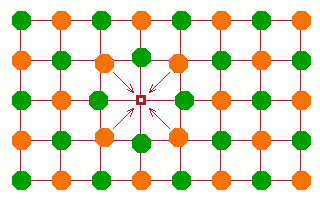
\includegraphics[width=0.25\textwidth]{vacancy}
        \centering
        \caption{Vacancy in a lattice}
    \end{figure}

    Another defect is the ``interstital particle''. This is when there is an
    ``extra'' particle in the lattice. This defect has a similar effect to a
    vacancy \cite{VirginiaDefects}.
    \begin{figure}[h]
        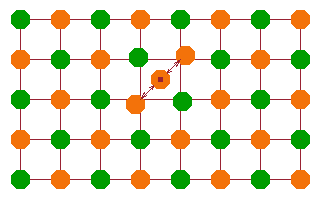
\includegraphics[width=0.25\textwidth]{interstital}
        \centering
        \caption{Interstital particle in a lattice}
    \end{figure}

    Both vacancies and interstital particles are highly mobile, and if they
    meet each other, they can ``annihilate'', or cancel each other out
    \cite{LatticeDefects}.

    Another type of lattice defect is an impurity - this is where ``a ``wrong''
    atom is placed on a regular lattice point'' \cite{LatticeDefects}.
    \begin{figure}[h]
        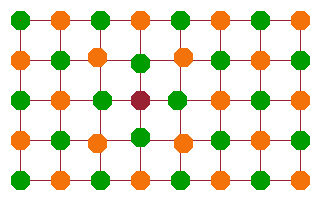
\includegraphics[width=0.25\textwidth]{impurity}
        \centering
        \caption{Impurity in a lattice}
    \end{figure}
\nocite{DoITPoMS}
\nocite{JimBook}
\nocite{HowItWorks}
\bibliography{metalsII}{}
\bibliographystyle{unsrt}
\end{document}
